
\documentclass[a4paper,11pt]{article}

\title{Documentation of SecLab System}

\usepackage[T1]{fontenc}
\usepackage{ae, aecompl}
\usepackage{a4wide}
\usepackage{boxedminipage}
\usepackage{url}
\usepackage{graphicx}
\usepackage{enumerate}
\usepackage{float}
\usepackage{multicol}
\usepackage{tabularx}



% Some useful commands and environments

\begin{document}
\title{Documentation of SecLab System}

\section{Network diagram}

\begin{figure}[H]
  \centering
    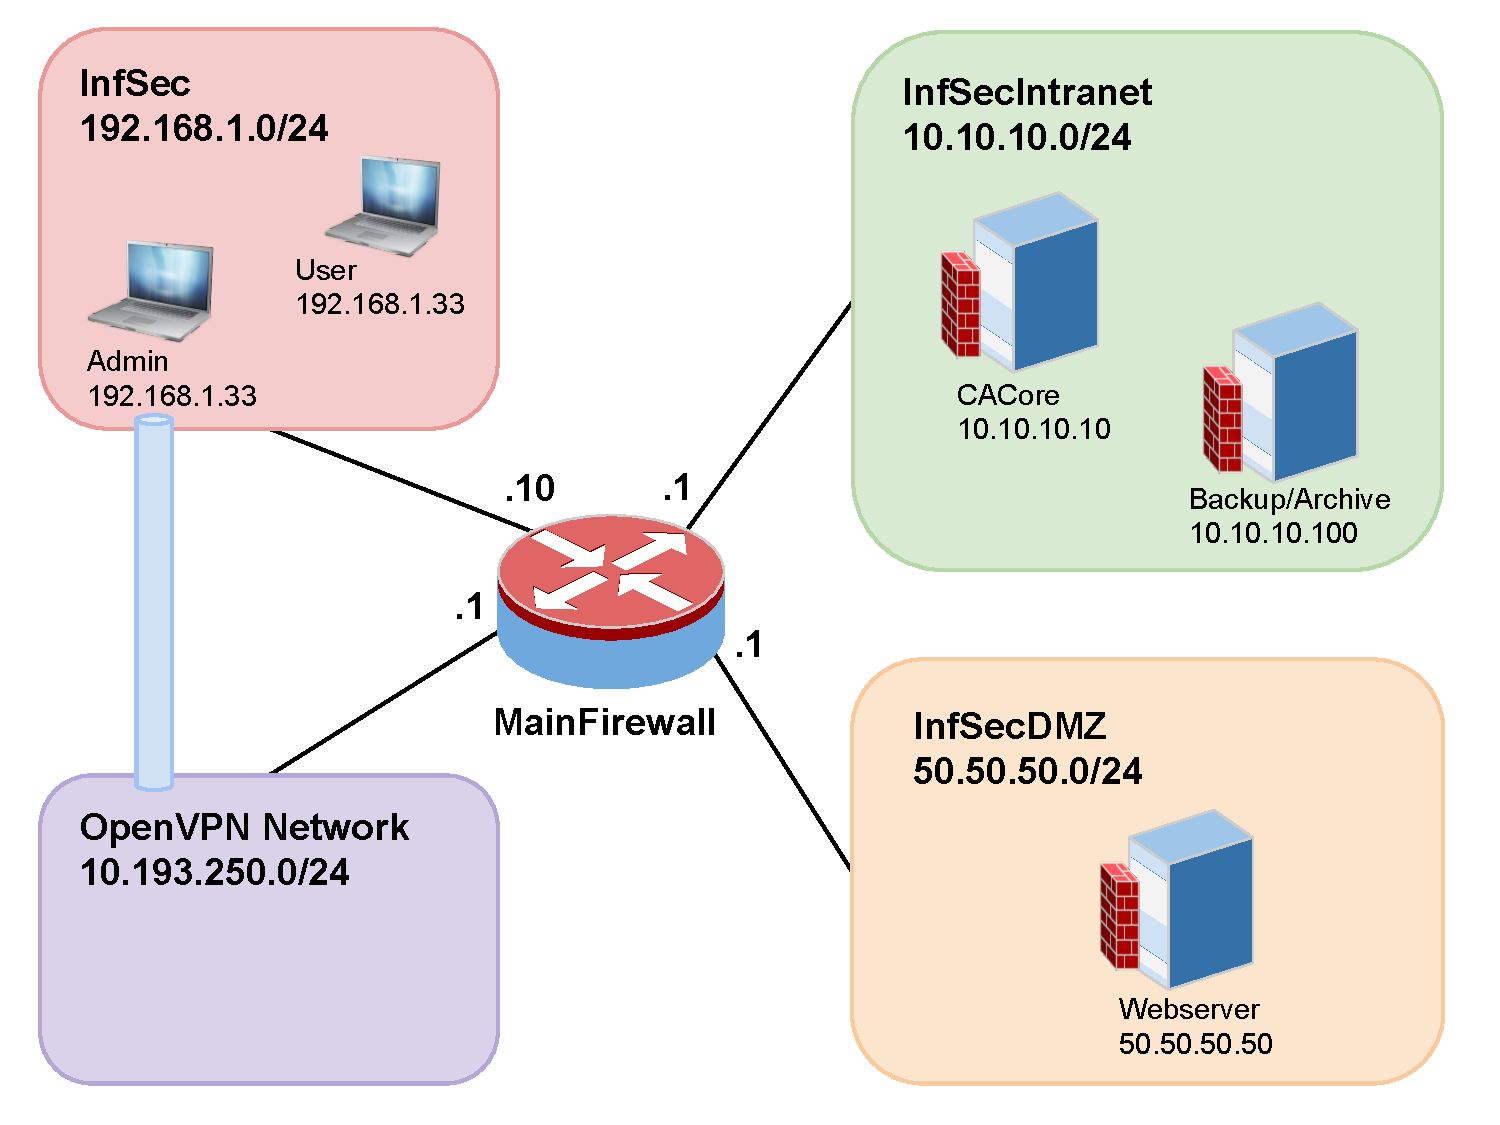
\includegraphics[width=0.9\textwidth]{sysseclab_net_diagram.pdf}  
  \caption{Network Diagram}
  \label{netdiag}
\end{figure}

\section{Servers}
All servers are equipped with at least one NIC corresponding to the network they are in as shown in Figure \ref{netdiag} and a NAT NIC that can be used for internet access (git, apt-get, etc.).
\subsection{MainFirewall}
\subsubsection*{Accounts \& Passwords}
\begin{multicols}{2}
\begin{description}
\item[admin:] wT7nDB7A7d7V
\item[root:] 5hmAMWxN6uVa
\end{description}
\end{multicols}
\subsubsection*{Installed software}
IPCop
\subsubsection*{User for ssh access}
Accesable only on 10.10.10.1 with port 8022 from 10.10.10.33 (user in InfSecIntranet) or from OpenVPN-Network.\newline
ssh -p 8022 admin@10.10.10.1
\subsubsection*{additional information}
There is a webinterface on https://10.10.10.1:8023. Only accessable from 10.10.10.33 (user in InfSecIntranet).

\subsection{Webserver}
\subsubsection*{Accounts \& Passwords}
\begin{multicols}{2}
\begin{description}
\item[serveruser:] 3FaVLt9RNxLu
\item[root:] cLepMVRq8wDQ
\end{description}
\end{multicols}
\subsubsection*{Installed software}
Debian, iptables, nginx, python, flask, openSSL, openSSH
\subsubsection*{Running services (lsof -i)}
sshd, nginx
\subsubsection*{User for ssh access}
ssh serveruser@50.50.50.50
\subsubsection*{additional information}
SSL signing key for HTTPS: 9klTRxBQcAnM

\subsection{CoreCA}
\subsubsection*{Accounts \& Passwords}
\begin{multicols}{2}
\begin{description}
\item[causer:] 9BxkXM5fLLL8
\item[root:] 8kSeddphG6Ac
\end{description}
\end{multicols}
\subsubsection*{Installed software}
Debian, iptables, python, mySQL, openSSL, openSSH
\subsubsection*{Running services (lsof -i)}
sshd, mysql (only localhost)
\subsubsection*{User for ssh access}
ssh causer@10.10.10.10
\subsubsection*{additional information}
MySQL root password: Cm7NsWBhf52C

\subsection{Backup/Archive Server}
\subsubsection*{Accounts \& Passwords}
\begin{multicols}{2}
\begin{description}
\item[archiveuser:] 4uMtrPMLxShw
\item[root:] gaBWUt5EH8vU
\end{description}
\end{multicols}
\subsubsection*{Installed software}
Debian, iptables, syslog, openSSH
\subsubsection*{Running services (lsof -i)}
sshd
\subsubsection*{User for ssh access}
ssh archiveuser@10.10.10.100

\subsection{User}
\subsubsection*{Accounts \& Passwords}
\begin{description}
\item[alice:] alice
\end{description}
\subsubsection*{additional information}
When running in netwok InfSec, VPN is possible (VPN start script on Desktop):\newline
\begin{description}
\item[PKCS12 PW:] StgmE58sadQu
\end{description}
When running in netwok InfSecIntranet, firewall web access on https://10.10.10.1:8023


\section{Firewall rules}
\subsection{MainFirewall}
All connections are closed by default. The following list shows the allowed exceptions:\newline

\begin{tabular}{l c l}
Source & Protocol & Destination \\
\cline{1-3}
Webserver & HTTPS (443) & InfSec \\
\cline{1-3}
InfSec & HTTPS (443) & Webserver \\
\cline{1-3}
10.10.10.33 & IPCop HTTPS (8023) & MainFirewall\\
\cline{1-3}
OpenVPN network & IPCop SSH (8022) & MainFirewall \\
\cline{1-3}
10.10.10.33 & IPCop SSH (8022) & MainFirewall \\
\cline{1-3}
BackupServer & IPCop SSH (8022) & MainFirewall \\
\cline{1-3}
OpenVPN network & SSH (22) & Backupserver \\
\cline{1-3}
OpenVPN network & SSH (22) & CACore \\
\cline{1-3}
OpenVPN network & SSH (22) & Webserver \\
\cline{1-3}
Webserver & RPC (4444) & CACore \\
\cline{1-3}
CACore & RPC (4444) & Webserver \\
\cline{1-3}
Backupserver & SSH (22) & Webserver \\
\end{tabular}

\subsection{Webserver}
All connections are closed by default. The following list shows the allowed exceptions:\newline


\begin{tabular}{c c c}
Source & Protocol & Destination \\
\cline{1-3}
Backupserver & SSH (22) & Webserver \\
\cline{1-3}
OpenVPN network & SSH (22) & Webserver \\
\cline{1-3}
InfSec & HTTPS (443) & Webserver \\
\cline{1-3}
CACore & RPC (4444) & Webserver \\
\cline{1-3}
Webserver & HTTPS (443) &  \\
\cline{1-3}
Webserver & RPC (4444) &  \\
\end{tabular}

\subsection{CoreCA}
All connections are closed by default. The following list shows the allowed exceptions:\newline


\begin{tabular}{c c c}
Source & Protocol & Destination \\
\cline{1-3}
Backupserver & SSH (22) & CACore \\
\cline{1-3}
OpenVPN network & SSH (22) & CACore \\
\cline{1-3}
Webserver & RPC (4444) & CACore \\
\cline{1-3}
CACore & RPC (4444) & Webserver \\
\cline{1-3}
CACore & SSH (22) & Backupserver \\
\end{tabular}

\subsection{Backup/Archive Server}
All connections are closed by default. The following list shows the allowed exceptions:\newline


\begin{tabular}{l c l}
Source & Protocol & Destination \\
\cline{1-3}
CACore & SSH (22) & Backupserver \\
\cline{1-3}
OpenVPN network & SSH (22) &  Backupserver\\
\cline{1-3}
Backupserver & SSH (22) & CACore \\
\cline{1-3}
Backupserver & SSH (22) & MainFirewall \\
\cline{1-3}
Backupserver & SSH (22) & Webserver \\
\end{tabular}

\end{document}
